\documentclass{beamer}
\usetheme{Antibes}
\setbeamertemplate{navigation symbols}{} 
\usefonttheme[onlymath]{serif}
\usepackage{amsmath}
\usepackage{lmodern}%
% \usepackage{showframe} 

\usepackage{graphicx}
\graphicspath{{.}{images/}}

\setbeamertemplate{caption}{\raggedright\insertcaption\par}

\title[Theoretical Optical Second-Harmonic Calculations for Surfaces
\hspace{5.5cm}\insertframenumber/\inserttotalframenumber]
{Theoretical Optical Second-Harmonic Calculations for Surfaces}
\author{\texorpdfstring{Sean M. Anderson\vspace{-0.7em}}{Sean M. Anderson}}
\institute{Centro de Investigaciones en \'Optica, A.C\vspace{-1em}}
\date{\small\today\vspace{-1.2em}}
\titlegraphic{
\begin{figure}
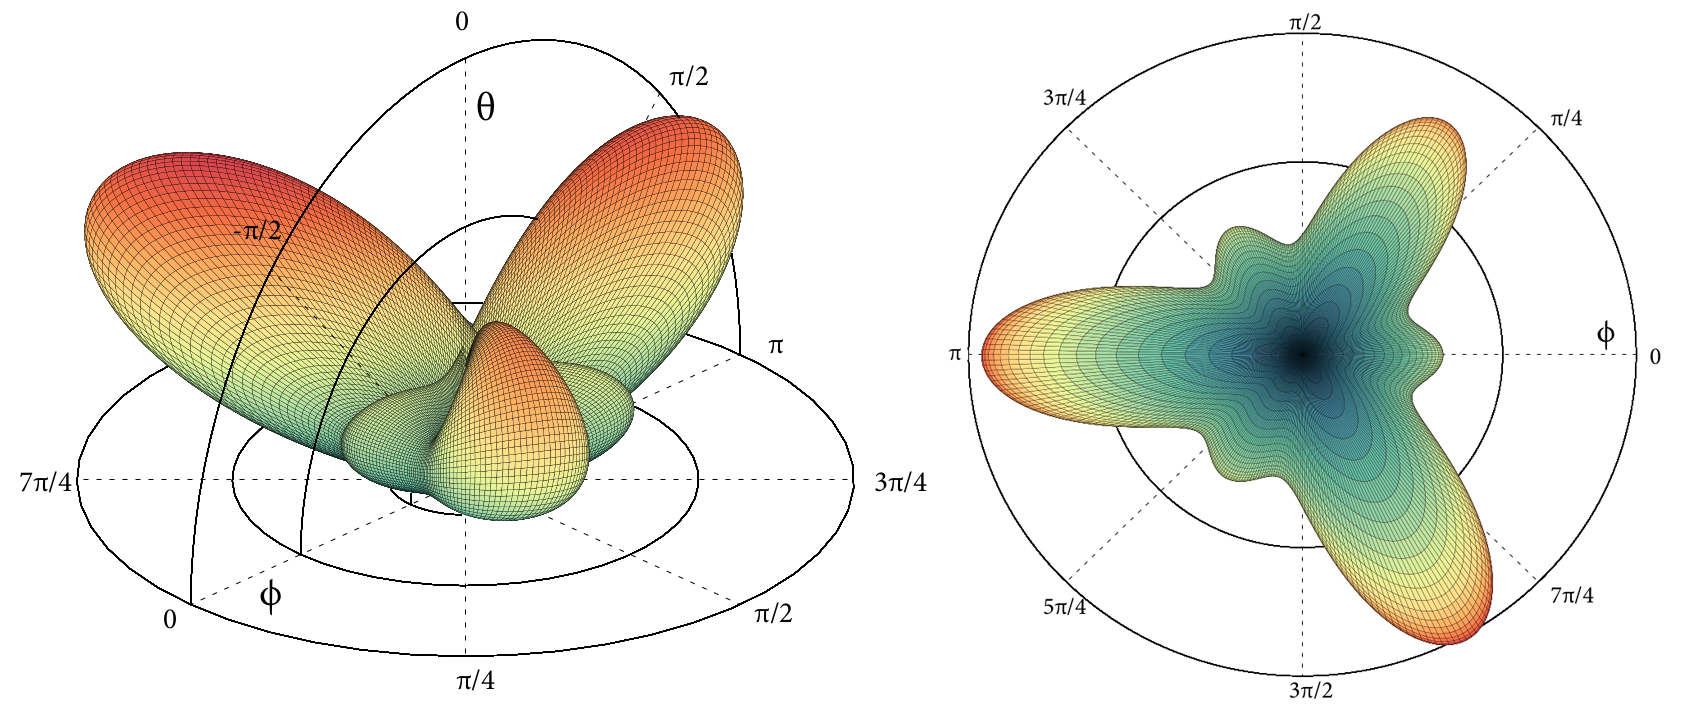
\includegraphics[width=0.8\textwidth]{3D-cover}
\end{figure}}


\begin{document}

\begin{frame}
\maketitle
\end{frame}

%%%%%%%%%%%%%%%%%%%%%%%%%%%%%%%%%%%%%%%%%%%%%%%%%%%%%%%%%%%%%%%%%%%%%%%%%%%%%%%%
%%%%%%%%%%%%%%%%%%%%%%%%%%%%%%%%%%%%%%%%%%%%%%%%%%%%%%%%%%%%%%%%%%%%%%%%%%%%%%%%

\section{Introduction}

\begin{frame}
\frametitle{Second Harmonic Generation (SHG)}
\begin{block}{Characteristics\footnote{Image: Jon Chui}}
\begin{itemize}
\item Two photons of the same frequency combine
\item Create one photon of double the frequency
\end{itemize}
\end{block}
\begin{figure}
\centering
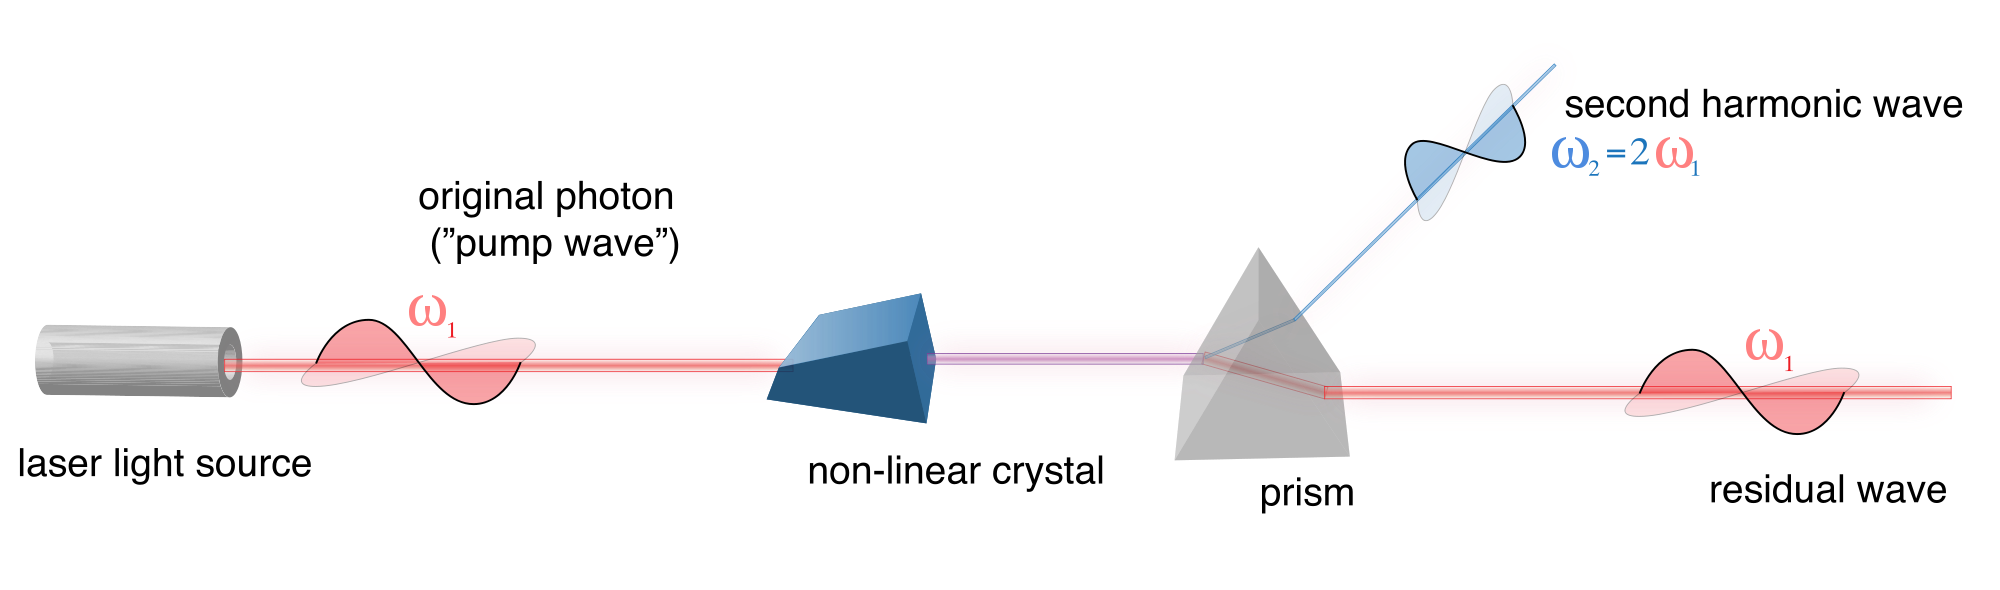
\includegraphics[width=0.9\textwidth]{diag-shg}
\end{figure}
\end{frame}

\begin{frame}
% \frametitle{A two column slide}
\begin{columns}
\column{0.5\textwidth}
\begin{figure}
\centering
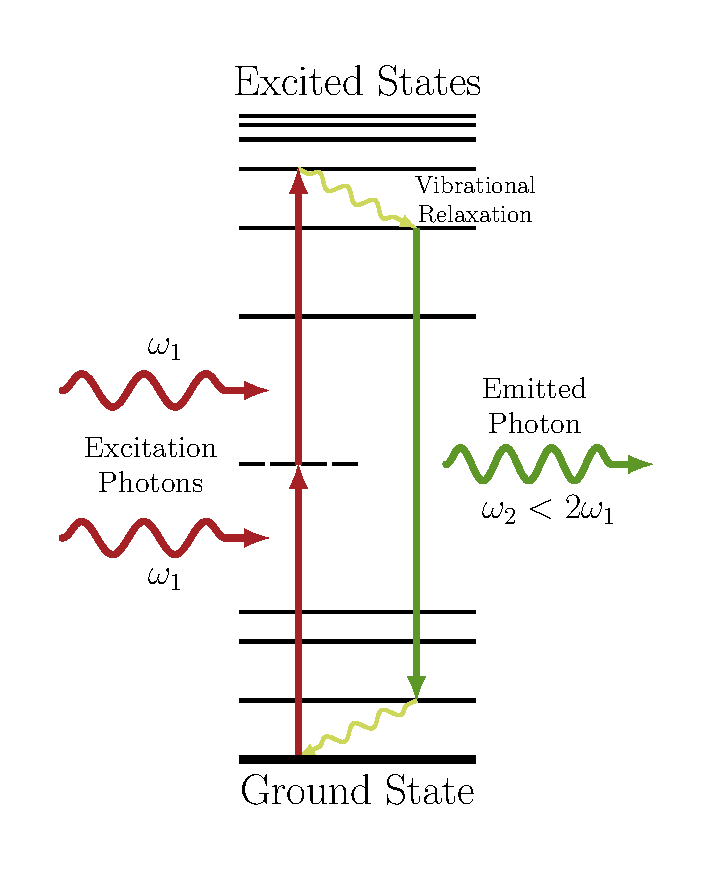
\includegraphics[width=\textwidth]{diag-levelsflourescence}
\end{figure}
\column{0.5\textwidth}
\begin{figure}
\centering
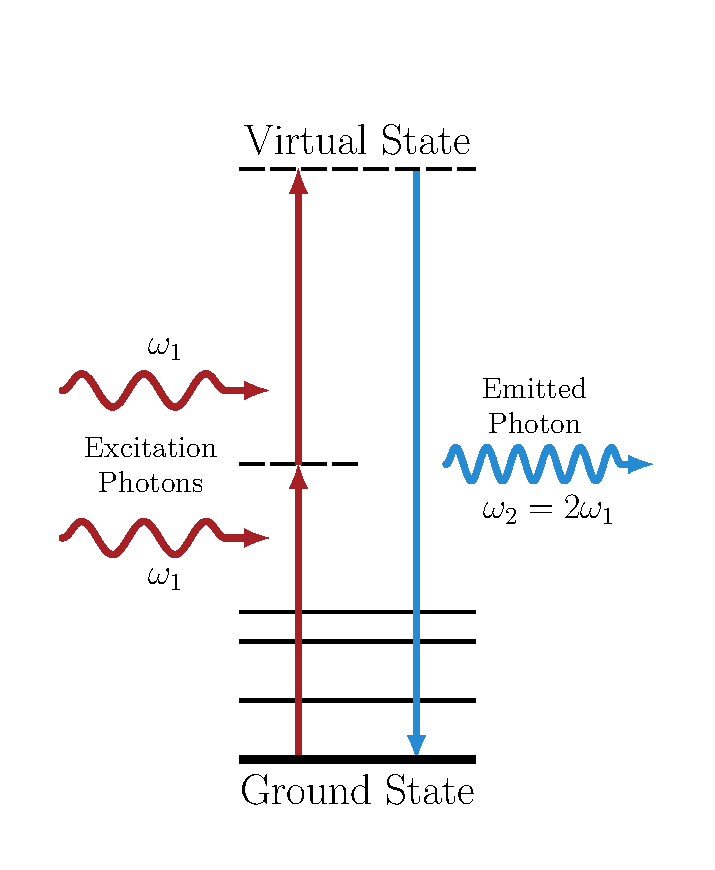
\includegraphics[width=\textwidth]{diag-levelsshg}
\end{figure}
\end{columns}
\end{frame}

\begin{frame}
\frametitle{Applications}
\begin{figure}
\centering
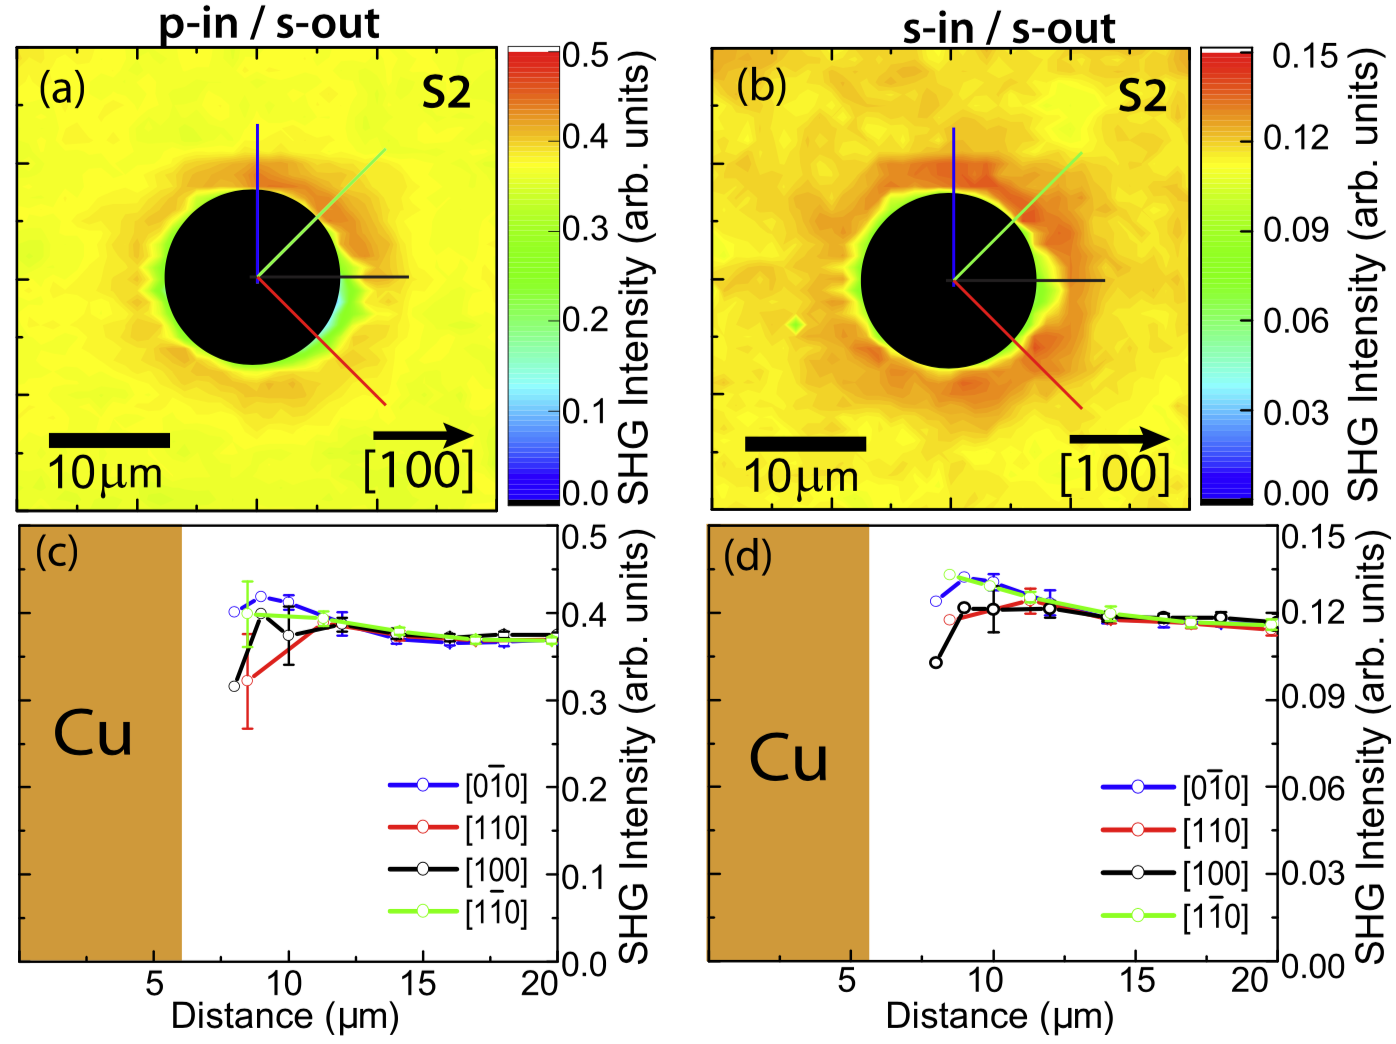
\includegraphics[width=0.6\textwidth]{image-yojin}
\caption{Test\footnote{\emph{Cho et al.}, Appl. Phys. Lett. 108, 151602 (2016)}}
\end{figure}
\end{frame}

\begin{frame}
\frametitle{Second-order Nonlinear Effects}
Second-order nonlinear processes\footnote{\emph{Armstrong et al.}, Phys. Rev.
127, 1918 (1962)}
\footnote{\emph{Bloembergen et al.}, Phys. Rev. 128, 606 (1962)}
\begin{itemize}
\item Are dipole forbidden in the bulk of centrosymmetric materials
\item Are related to $\chi^{(2)}$, the nonlinear susceptibility
\item Have bigger dipolar (surface) than quadrupolar contributions
\end{itemize}
\end{frame}

\begin{frame}
\frametitle{Centrosymmetric Materials}
A centrosymmetric material is a material that displays inversion symmetry, such
that $p(a,b,c) \rightarrow p(-a,-b,-c)$.
\begin{figure}
\centering
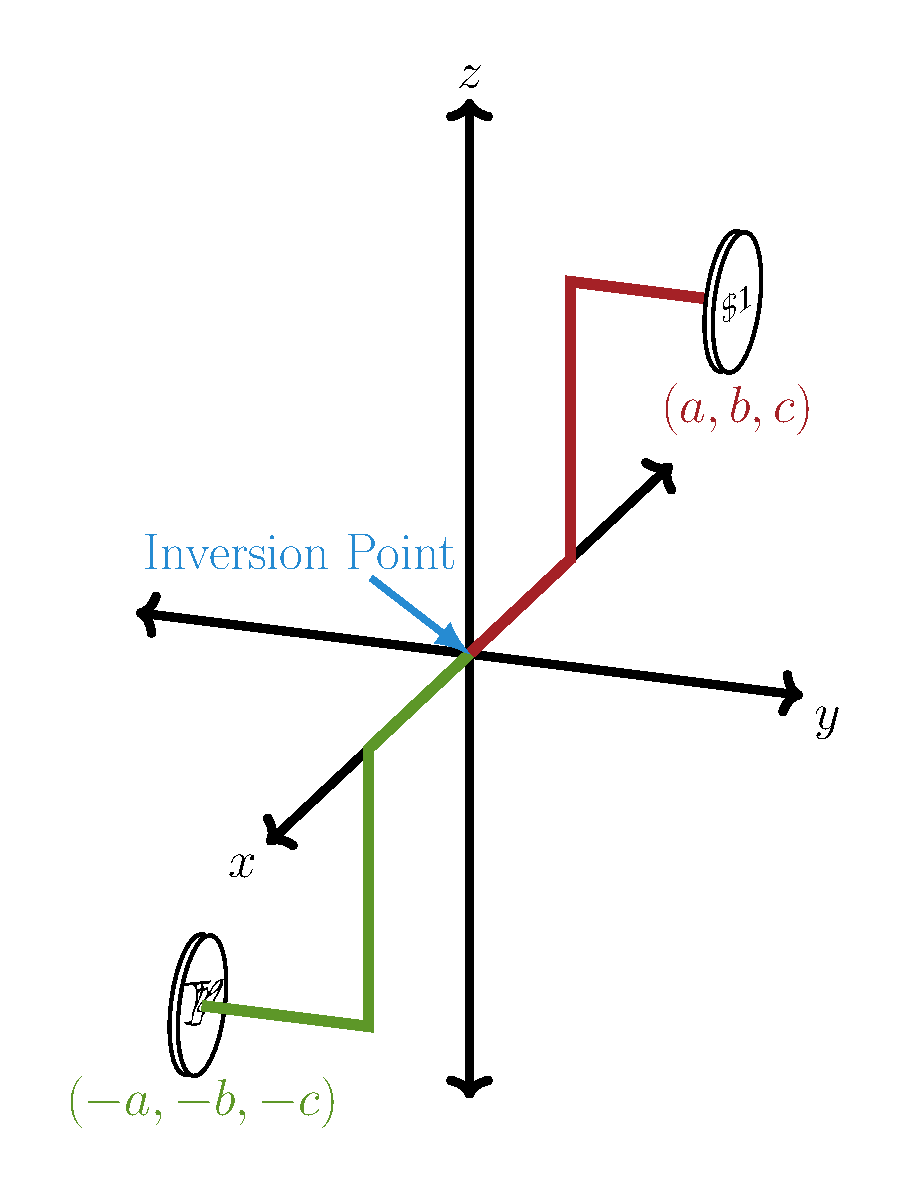
\includegraphics[height=0.7\textheight]{diag-centrosymmetry}
\end{figure}
\end{frame}

\begin{frame}
% \frametitle{A two column slide}
\begin{figure}
\centering
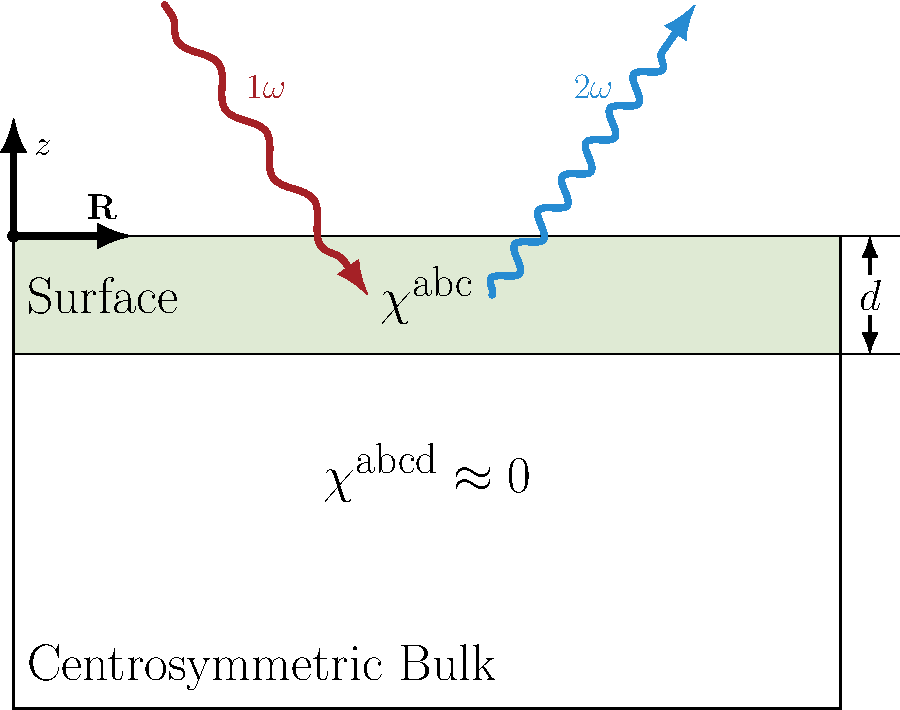
\includegraphics[width=\textwidth]{diag-system}
\end{figure}
\end{frame}

\begin{frame}
\frametitle{Test Cases}
\begin{columns}
\column{0.5\textwidth}
\begin{figure}
\centering
\includegraphics[height=0.7\textheight]{struc-Si2x1-front}
\caption{Si(001)(2$\times$1)}
\end{figure}
\column{0.5\textwidth}
\begin{figure}
\centering
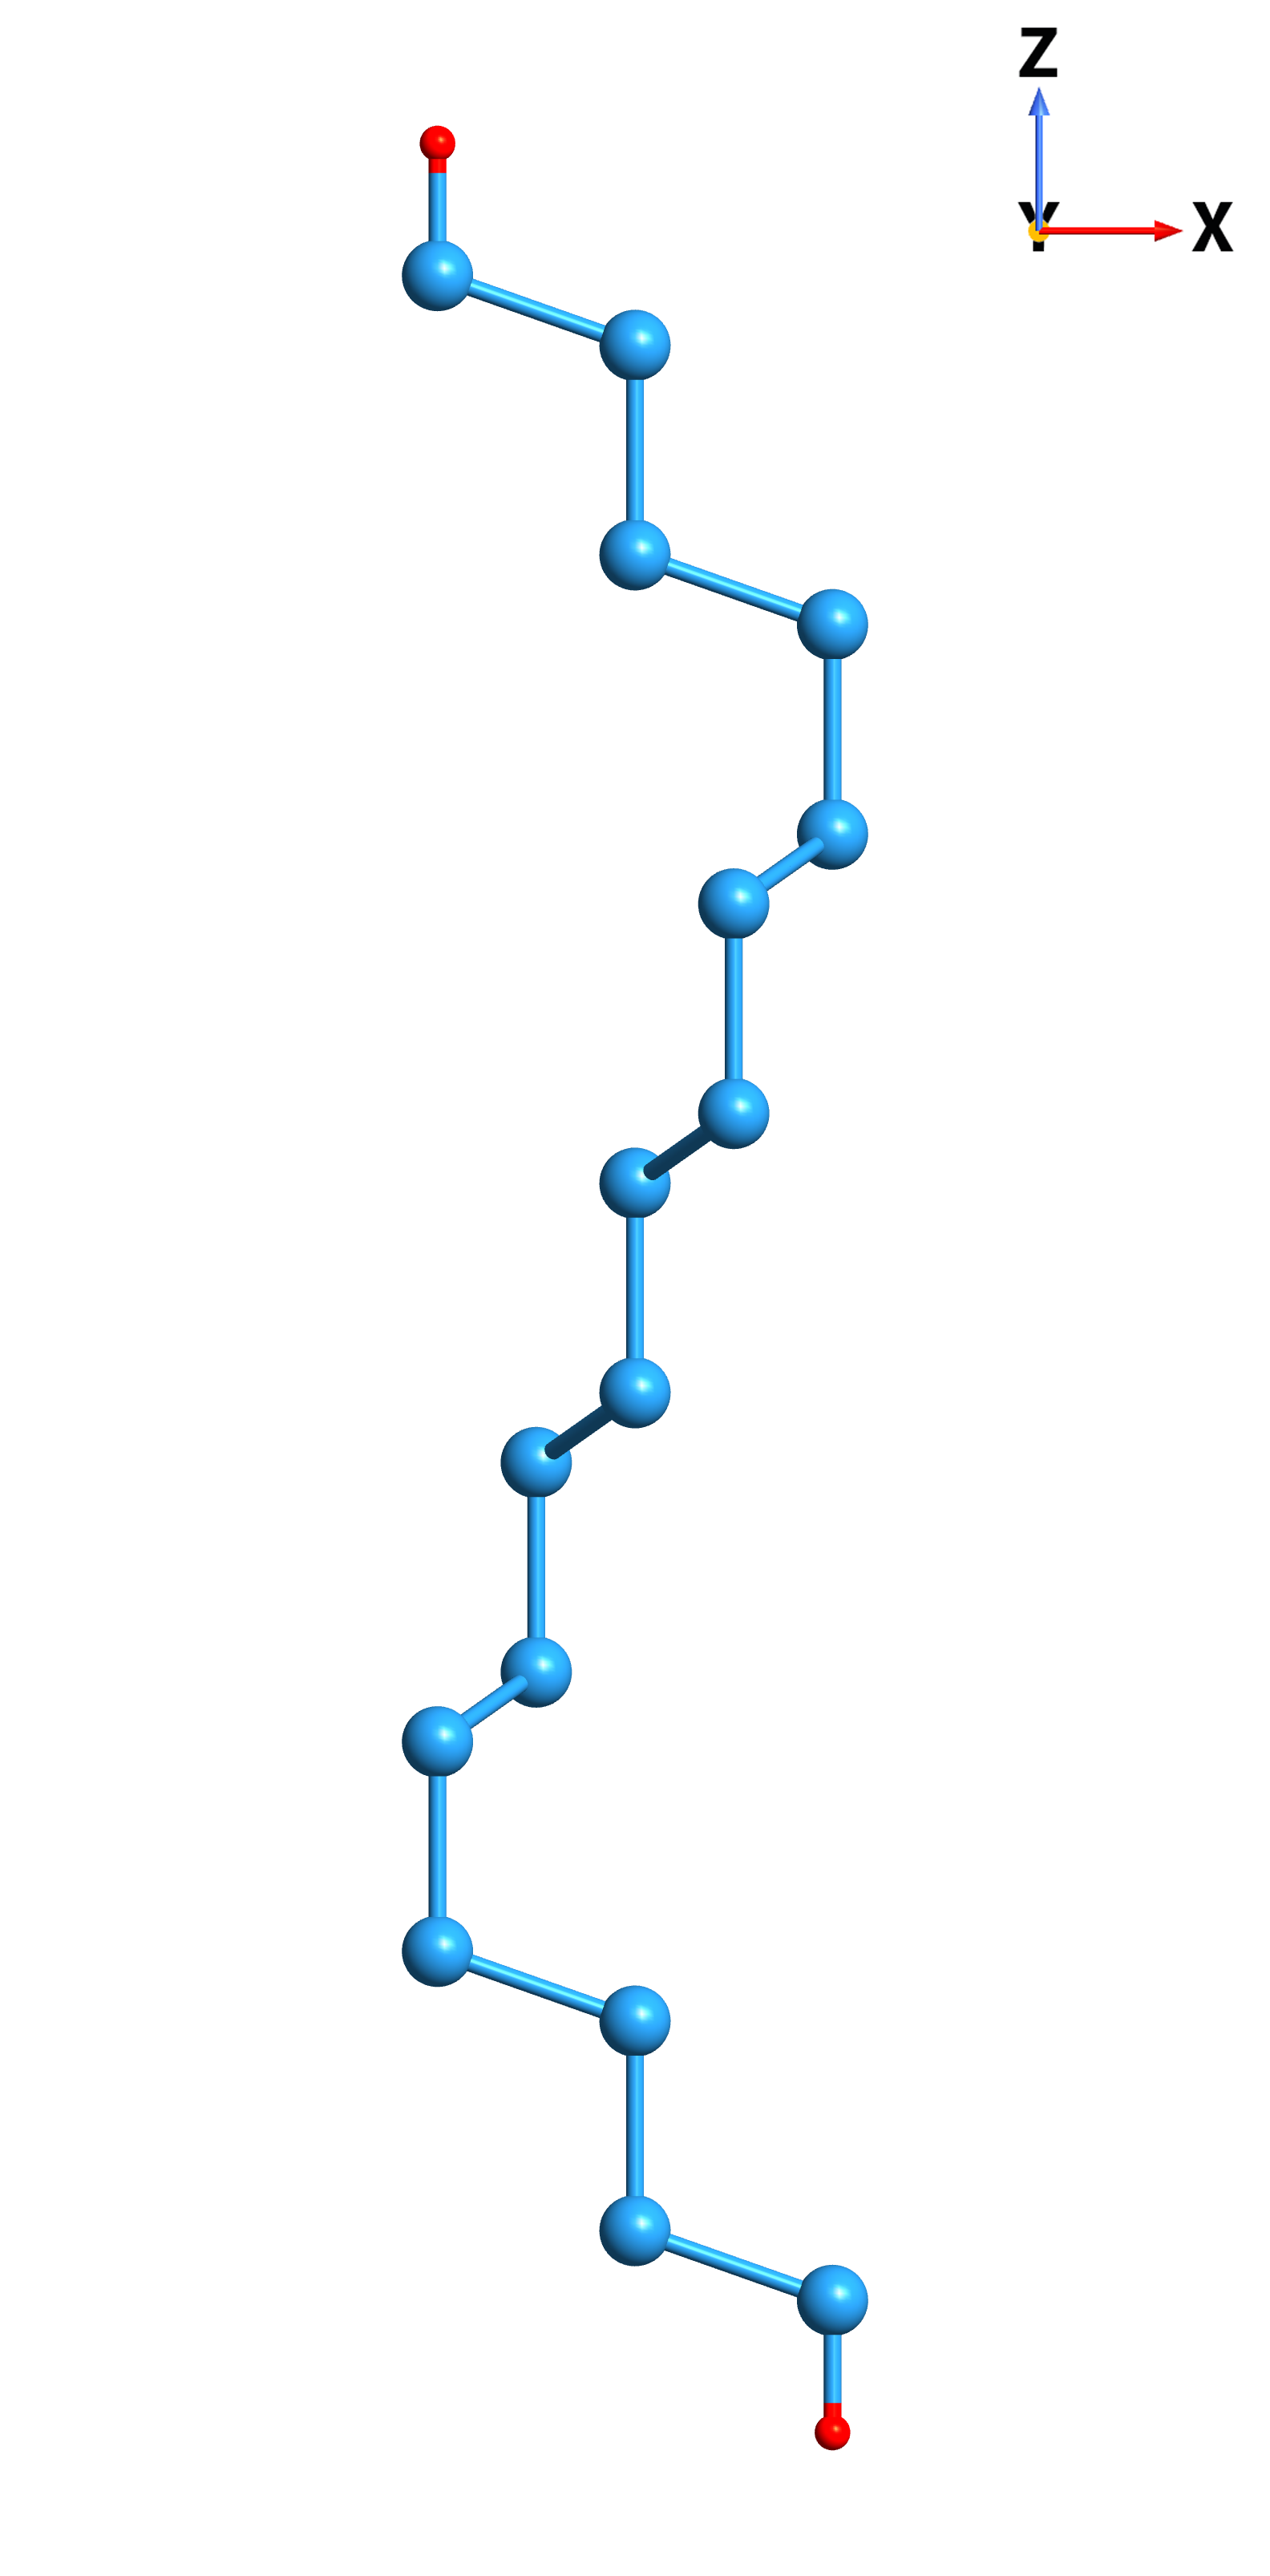
\includegraphics[height=0.7\textheight]{struc-Si1x1-front}
\caption{Si(111)(1$\times$1):H}
\end{figure}
\end{columns}
\end{frame}


%%%%%%%%%%%%%%%%%%%%%%%%%%%%%%%%%%%%%%%%%%%%%%%%%%%%%%%%%%%%%%%%%%%%%%%%%%%%%%%%
%%%%%%%%%%%%%%%%%%%%%%%%%%%%%%%%%%%%%%%%%%%%%%%%%%%%%%%%%%%%%%%%%%%%%%%%%%%%%%%%

\section{The Nonlinear Surface Susceptibility}


%%%%%%%%%%%%%%%%%%%%%%%%%%%%%%%%%%%%%%%%%%%%%%%%%%%%%%%%%%%%%%%%%%%%%%%%%%%%%%%%

\subsection{Nonlocal Operators}

\begin{frame}
Our new formulation adds three contributions:%
\footnote{\emph{Anderson et al.}, Phys. Rev. B. 91, 075302 (2015)}
\begin{enumerate}
\item The scissors correction
\item The contribution from the nonlocal part of the pseudopotential
\item The layered cut function
\end{enumerate}
\end{frame}

\begin{frame}
\frametitle{Scissors Operator and
\texorpdfstring{$\mathbf{v}^{\mathrm{nl}}$}{vnl} (1 \& 2)} We express the
electron velocity operator as
\begin{equation*}\label{vop2}
\begin{split}
\mathbf{v}^{\Sigma}
&=\mathbf{v} + \mathbf{v}^{\mathrm{nl}} 
+ \mathbf{v}^{\mathcal{S}}
= \mathbf{v}^\mathrm{LDA} + \mathbf{v}^{\mathcal{S}},
\end{split}
\end{equation*}
which includes the nonlocal part of the pseudopotential and the scissors
correction, where
\begin{equation*}\label{conhr}
\begin{split}
\mathbf{v} &=\frac{\mathbf{p}}{m_{e}},\\
\mathbf{v}^{\mathrm{nl}} &= \frac{1}{i\hbar}
  \left[\mathbf{r},V^{\mathrm{nl}}\right],\\
\mathbf{v}^{\mathcal{S}} &= \frac{1}{i\hbar}
  \left[\mathbf{r},S(\mathbf{r},\mathbf{p})\right],\\
\mathbf{v}^\mathrm{LDA} &= \mathbf{v}+\mathbf{v}^{\mathrm{nl}}.
\end{split}
\end{equation*}  
\end{frame}


%%%%%%%%%%%%%%%%%%%%%%%%%%%%%%%%%%%%%%%%%%%%%%%%%%%%%%%%%%%%%%%%%%%%%%%%%%%%%%%%

\subsection{Layered Cut Function}

\begin{frame}
\frametitle{Layered Cut Function (3)}
We introduce the cut function
\begin{equation*}
{\boldsymbol{\mathcal{C}}}(z)=\Theta(z-z_\ell+\Delta_\ell^{b})  
            \Theta(z_\ell-z+\Delta_\ell^f),
\label{sz}
\end{equation*}
that transforms any operator into its calligraphic counterpart as
\begin{equation*}
\mathbf{V} \to \boldsymbol{\mathcal{V}}
= \frac{\boldsymbol{\mathcal{C}}(z) \mathbf{V}
+ \mathbf{V} \boldsymbol{\mathcal{C}}(z)}{2},
\label{vcali}
\end{equation*} 
\end{frame}

\begin{frame}
\frametitle{Layered Cut Function (3)}
\begin{figure}
\centering
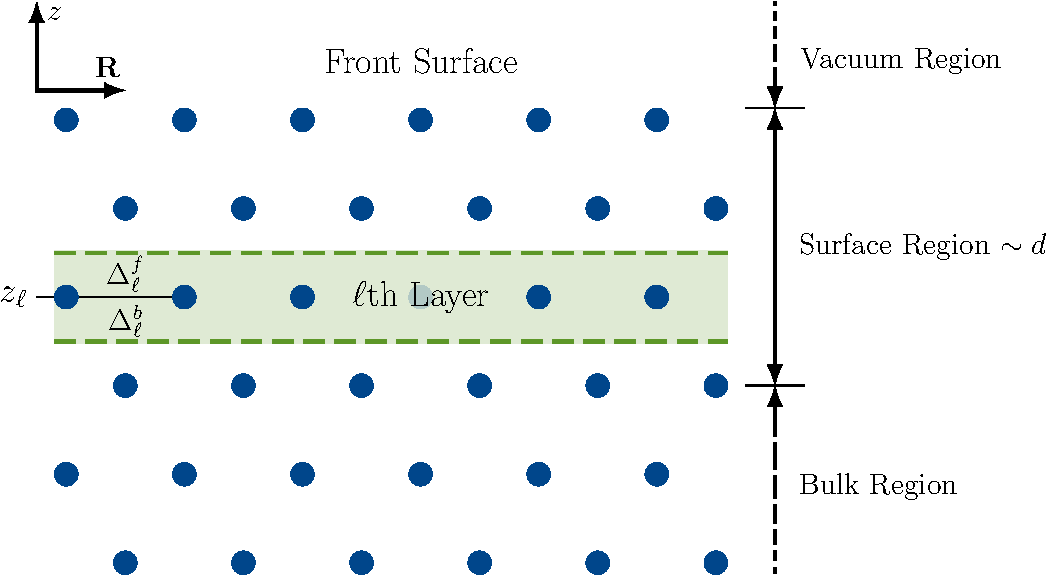
\includegraphics[width=0.9\textwidth]{diag-slab}
\caption{Sketch of the super-cell. The atomic slab corresponds to the circles
representing the atoms of the system.}
\end{figure}
\end{frame}

%%%%%%%%%%%%%%%%%%%%%%%%%%%%%%%%%%%%%%%%%%%%%%%%%%%%%%%%%%%%%%%%%%%%%%%%%%%%%%%%

\subsection{Summary}

\begin{frame}
\frametitle{Final Expressions}
\begin{block}{Interband Contribution}
\begin{figure}
\centering
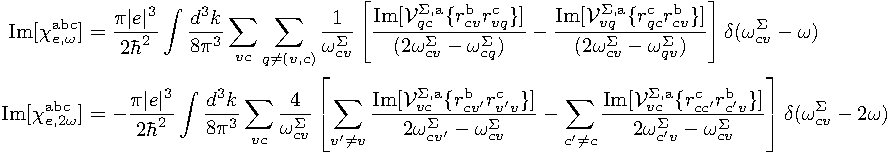
\includegraphics[scale=0.70]{chis_inter}
\end{figure}
\end{block}
\begin{alertblock}{Intraband Contribution}
\begin{figure}
\centering
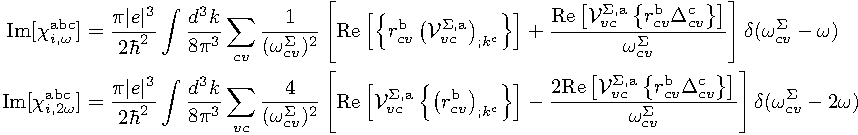
\includegraphics[scale=0.70]{chis_intra}
\end{figure}
\end{alertblock}
\end{frame}

\begin{frame}
\frametitle{Coding}
abinit, DP, tiniba
\end{frame}

%%%%%%%%%%%%%%%%%%%%%%%%%%%%%%%%%%%%%%%%%%%%%%%%%%%%%%%%%%%%%%%%%%%%%%%%%%%%%%%%

\subsection{Results for \texorpdfstring{$\boldsymbol{\chi}$}{X}:
\texorpdfstring{Si(001)(2$\times$1)}{Si(001)(2x1)}}

\begin{frame}
\frametitle{The Si(001)(2$\times$1) Slab}
\begin{figure}
\centering
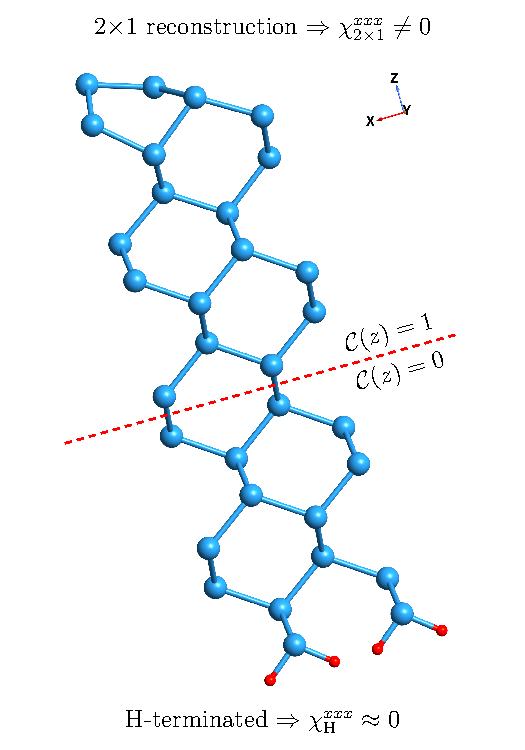
\includegraphics[height=0.7\textheight]{struc-Si2x1-rot}
\caption{Convergence is achieved with 32 layers of Si.}
\end{figure}
\end{frame}

\begin{frame}
\frametitle{Half-slab vs. Full-slab}
\begin{figure}
\centering
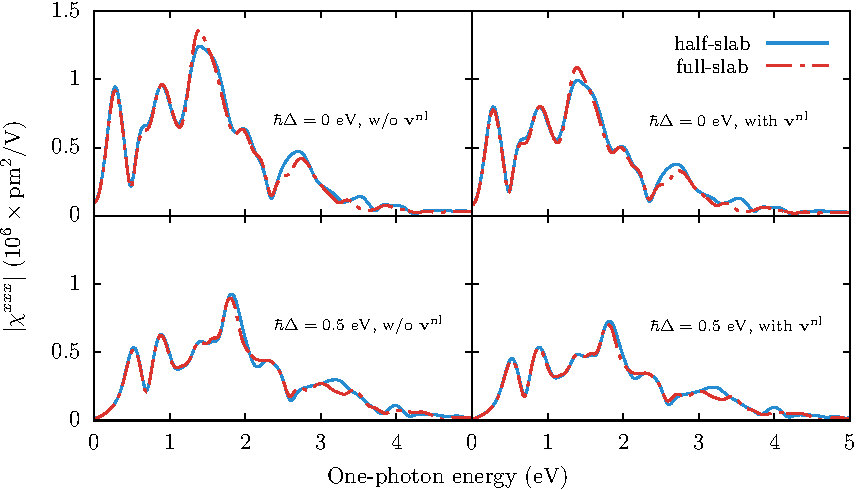
\includegraphics[width=0.9\textwidth]{fig-Si2x1-hsvsfs}
\caption{More layers would produce even better results.}
\end{figure}
\end{frame}

\begin{frame}
\frametitle{oh snap mofo}
\begin{figure}
\centering
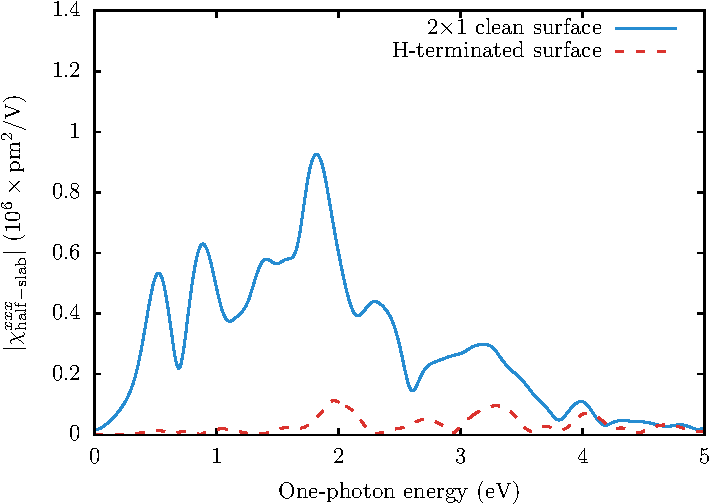
\includegraphics[width=0.9\textwidth]{fig-Si2x1-topvbottom}
\caption{wait until calc finishes yo}
\end{figure}
\end{frame}

\begin{frame}
\frametitle{Three Values of the Scissors Correction}
\begin{figure}
\centering
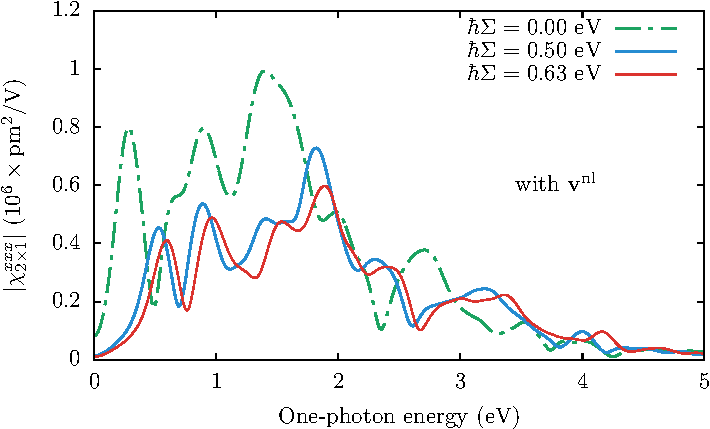
\includegraphics[width=0.9\textwidth]{fig-Si2x1-scissors}
\caption{The 2$\times$1 reconstructed surface has surface states, so the
spectrum shifts non-rigidly.}
\end{figure}
\end{frame}

\begin{frame}
\frametitle{With and Without \texorpdfstring{$\mathbf{v}^{\mathrm{nl}}$}{vnl}}
\begin{figure}
\centering
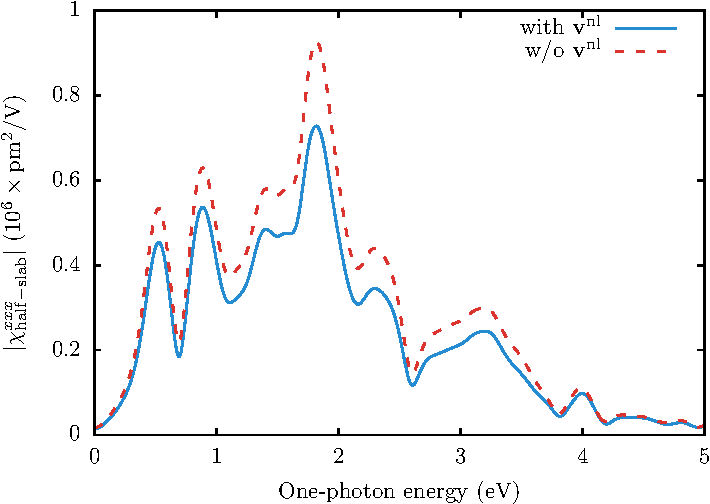
\includegraphics[width=0.9\textwidth]{fig-Si2x1-vnl}
\caption{The effect of the nonlocal part of the pseudopotentials maintains the
same line-shape but reduces the value of by 15-20\%.}
\end{figure}
\end{frame}


%%%%%%%%%%%%%%%%%%%%%%%%%%%%%%%%%%%%%%%%%%%%%%%%%%%%%%%%%%%%%%%%%%%%%%%%%%%%%%%%

\subsection{Results for \texorpdfstring{$\boldsymbol{\chi}$}{X}:
\texorpdfstring{Si(111)(1$\times$1):H}{Si(111)(1x1):H}}

\begin{frame}
\frametitle{$\boldsymbol{\chi}$ for the Si(111)(1$\times$1):H surface%
\footnote{Experimental data from Appl. Phys. A 63, 533 (1996)}}
\begin{figure}
\centering
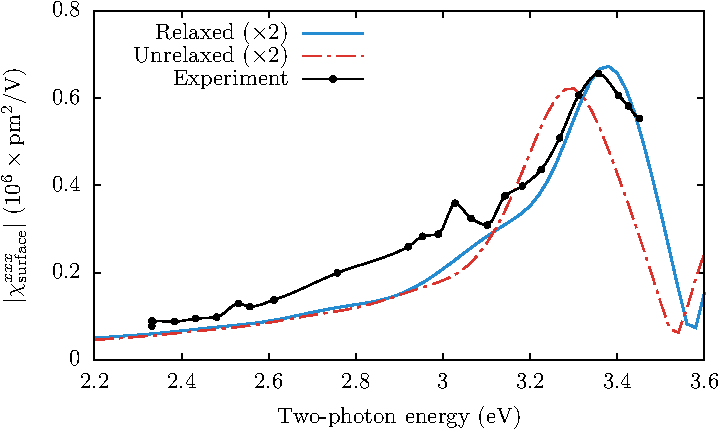
\includegraphics[width=0.5\textwidth]{fig-Si1x1-Hofer_Xxxx}
\end{figure}
\begin{block}{Relaxing the Structure}
\begin{enumerate}
\item Worth the time and effort
\item We'll talk about temp later
\end{enumerate}
\end{block}
\end{frame}


%%%%%%%%%%%%%%%%%%%%%%%%%%%%%%%%%%%%%%%%%%%%%%%%%%%%%%%%%%%%%%%%%%%%%%%%%%%%%%%%
%%%%%%%%%%%%%%%%%%%%%%%%%%%%%%%%%%%%%%%%%%%%%%%%%%%%%%%%%%%%%%%%%%%%%%%%%%%%%%%%

\section{The SSHG Yield}


%%%%%%%%%%%%%%%%%%%%%%%%%%%%%%%%%%%%%%%%%%%%%%%%%%%%%%%%%%%%%%%%%%%%%%%%%%%%%%%%

\subsection{The Three Layer Model}

\begin{frame}
% \frametitle{A two column slide}
\begin{figure}
\centering
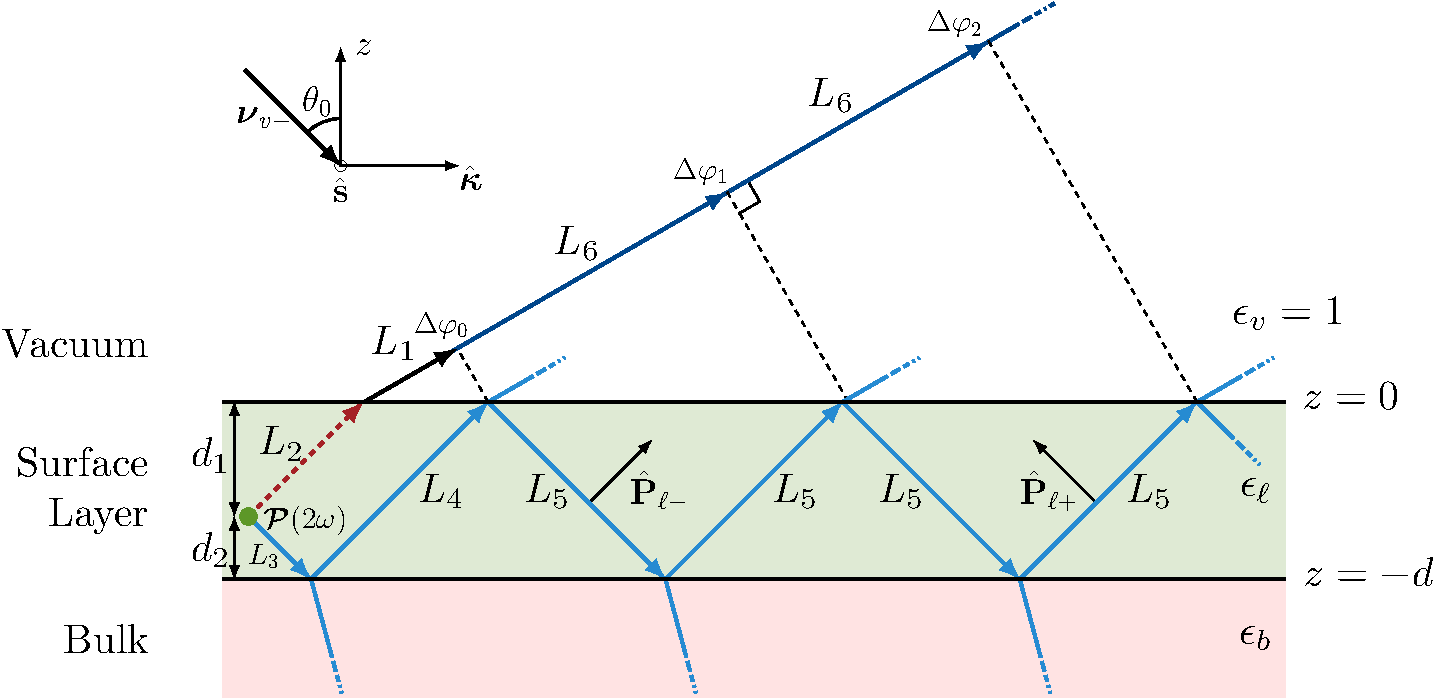
\includegraphics[width=\textwidth]{diag-3layer_MR_2w}
\end{figure}
\end{frame}


%%%%%%%%%%%%%%%%%%%%%%%%%%%%%%%%%%%%%%%%%%%%%%%%%%%%%%%%%%%%%%%%%%%%%%%%%%%%%%%%

\subsection{Explicit Expressions for \texorpdfstring{$\mathcal{R}$}{R}}

\begin{frame}
\frametitle{Explicit Expressions for $\mathcal{R}$}
The SSHG yield is
\begin{equation*}
\mathcal{R}_{\mathrm{iF}}(2\omega) =
\frac{\omega^{2}}{2\epsilon_{0}c^3\cos^{2}\theta_{0}}
\left\vert\frac{1}{n_{\ell}}\Upsilon_{\mathrm{iF}}\right\vert^{2} 
\end{equation*}
for each combination of polarizations of incoming and outgoing fields ($\mathrm{iF} = pP,
pS, sP,$ and $sS$). We have that
\begin{equation*}\label{eq:mc25}
\Upsilon_{\mathrm{iF}} = \Gamma_{\mathrm{iF}}\,r_{\mathrm{iF}},
\end{equation*}
where,
$$
\begin{array}{ l l }
\Gamma_{pP} =
\frac{T^{v\ell}_{p}}{N_{\ell}}
\left(\frac{t^{v\ell}_{p}}{n_{\ell}}\right)^{2},
&
\Gamma_{sP}=
\frac{T^{v\ell}_{p}}{N_{\ell}}
\left(t^{v\ell}_{s}r^{M+}_{s}\right)^{2},\quad\\
\Gamma_{pS} =
T_{s}^{v\ell}R^{M+}_{s}
\left(\frac{t^{v\ell}_{p}}{n_{\ell}}\right)^{2},\quad
&
\Gamma_{sS} = 
T_{s}^{v\ell}R^{M+}_{s}\left(t^{v\ell}_{s}r^{M+}_{s}\right)^{2},
\end{array}
$$
\end{frame}

\begin{frame}
\frametitle{Explicit Expressions for $\mathcal{R}$}
In particular, for the (111) surface we have
\begin{align*}
r^{(111)}_{pP} &= 
R^{M+}_{p}\sin\theta_{0}
\Big[
  \left(r^{M+}_{p}\right)^{2}\sin^{2}\theta_{0}\chi^{zzz}
+ \left(r^{M-}_{p}\right)^{2}w^{2}_{\ell}\chi^{zxx}
\Big]\\
&- R^{M-}_{p}w_{\ell}W_{\ell}
\Big[
  2r^{M+}_{p}r^{M-}_{p}\sin\theta_{0}\chi^{xxz}
+ \left(r^{M-}_{p}\right)^{2}w_{\ell}\chi^{xxx}\cos3\phi
\Big],\\\\
r^{(111)}_{sP} &= 
R^{M+}_{p}\sin\theta_{0}\chi^{zxx} +
R^{M-}_{p}W_{\ell}\chi^{xxx}\cos3\phi,\\\\
r^{(111)}_{pS} &= - \left(r^{M-}_{p}\right)^{2}w^{2}_{\ell}\chi^{xxx}\sin3\phi,\\\\
r^{(111)}_{sS} &= \chi^{xxx}\sin3\phi.
\end{align*}
\end{frame}

\begin{frame}
\frametitle{About the Code}
python, shgyield.py, github, robustness
\end{frame}


%%%%%%%%%%%%%%%%%%%%%%%%%%%%%%%%%%%%%%%%%%%%%%%%%%%%%%%%%%%%%%%%%%%%%%%%%%%%%%%%

\subsection{Results for \texorpdfstring{$\mathcal{R}$}{R}: 
Si(111)(1\texorpdfstring{$\times$}{x}1):H}

\begin{frame}
\frametitle{Si(111)(1\texorpdfstring{$\times$}{x}1):H -- Outgoing
\texorpdfstring{$P$}{P} polarization}
\begin{columns}
\column{0.55\textwidth}
\begin{figure}
\centering
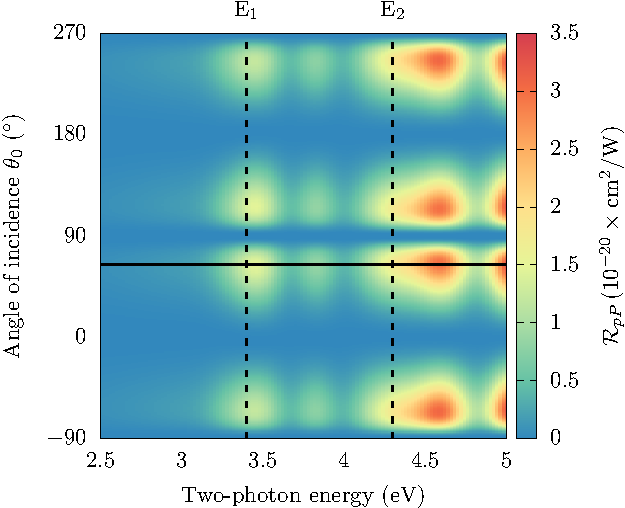
\includegraphics[width=\textwidth]{3D-Si1x1-RpP}
\caption{$\mathcal{R}_{pP}$}
\end{figure}
\column{0.55\textwidth}
\begin{figure}
\centering
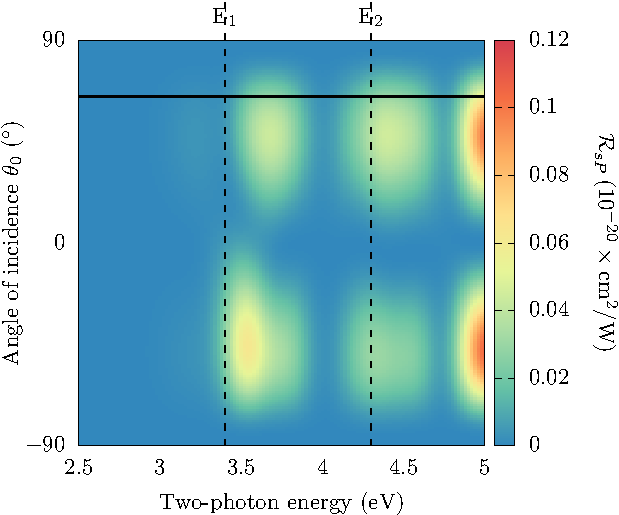
\includegraphics[width=\textwidth]{3D-Si1x1-RsP}
\caption{$\mathcal{R}_{sP}$}
\end{figure}
\end{columns}
\end{frame}

\begin{frame}
\frametitle{Si(111)(1\texorpdfstring{$\times$}{x}1):H -- Outgoing
\texorpdfstring{$S$}{S} polarization}
\begin{columns}
\column{0.55\textwidth}
\begin{figure}
\centering
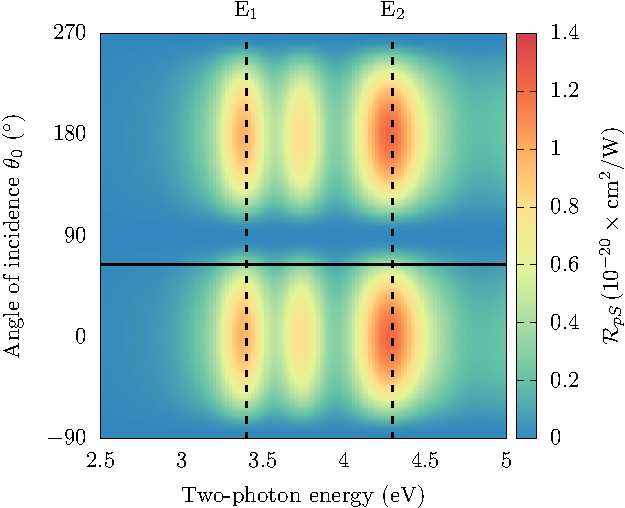
\includegraphics[width=\textwidth]{3D-Si1x1-RpS}
\caption{$\mathcal{R}_{pS}$}
\end{figure}
\column{0.55\textwidth}
\begin{figure}
\centering
\includegraphics[width=\textwidth]{3D-Si1x1-RsS}
\caption{$\mathcal{R}_{sS}$}
\end{figure}
\end{columns}
\end{frame}

\begin{frame}
% \frametitle{A two column slide}
\begin{figure}
\centering
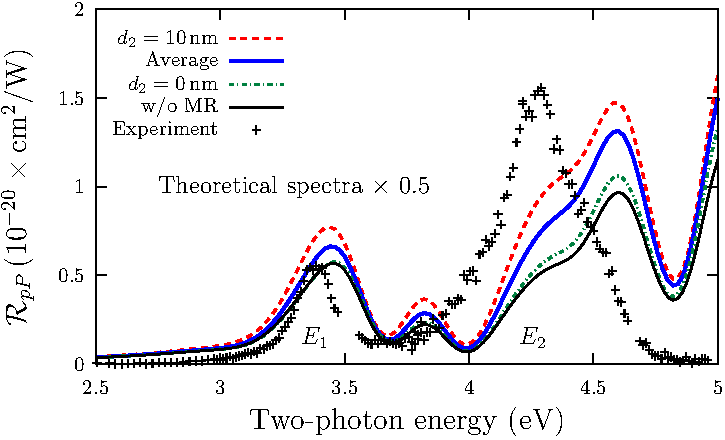
\includegraphics[width=0.9\textwidth]{fig-Si1x1-MRdepth}
\end{figure}
\end{frame}

\begin{frame}
% \frametitle{A two column slide}
\begin{figure}
\centering
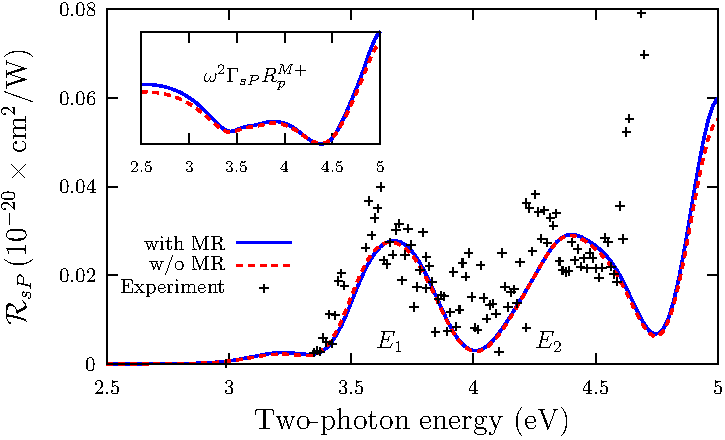
\includegraphics[width=\textwidth]{fig-Si1x1-Mejia_RsP}
\end{figure}
\end{frame}

\begin{frame}
% \frametitle{A two column slide}
\begin{figure}
\centering
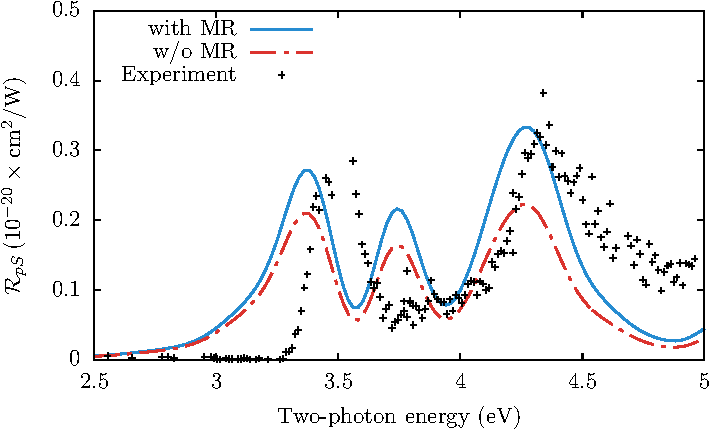
\includegraphics[width=\textwidth]{fig-Si1x1-Mejia_RpS}
\end{figure}
\end{frame}


%%%%%%%%%%%%%%%%%%%%%%%%%%%%%%%%%%%%%%%%%%%%%%%%%%%%%%%%%%%%%%%%%%%%%%%%%%%%%%%%
%%%%%%%%%%%%%%%%%%%%%%%%%%%%%%%%%%%%%%%%%%%%%%%%%%%%%%%%%%%%%%%%%%%%%%%%%%%%%%%%

\section{Conclusions}

\subsection{Chi2}
\begin{frame}
\frametitle{Title}
\begin{itemize}
\item Item 1
\item Item 2
\item Item 3
\end{itemize}
\end{frame}

\begin{frame}
Some starting text,
\begin{equation*}
E = mc^{2},
\end{equation*}
and more text.
\begin{block}{A block}
\begin{itemize}
\item Item 1
\item Item 2
\end{itemize}
\end{block}
\end{frame}

\begin{frame}
% \frametitle{A two column slide}
\begin{figure}
\centering
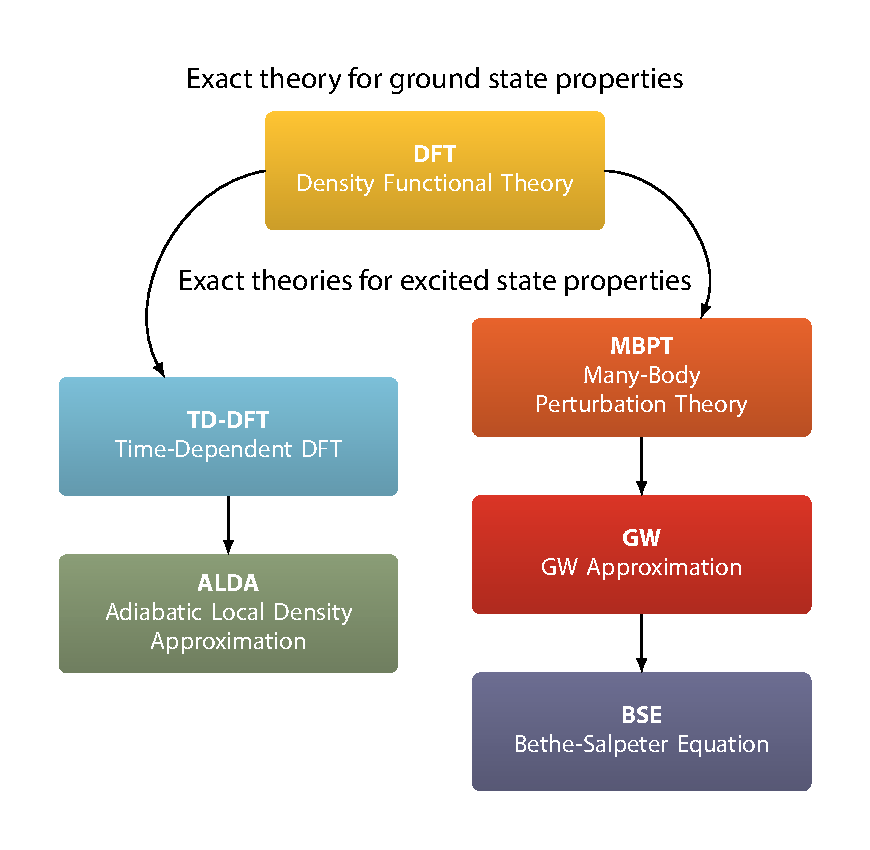
\includegraphics[height=\textheight]{diag-methods}
\end{figure}
\end{frame}

\begin{frame}
\frametitle{Appendix}
\begin{columns}
\column{0.5\textwidth}
\begin{figure}
\centering
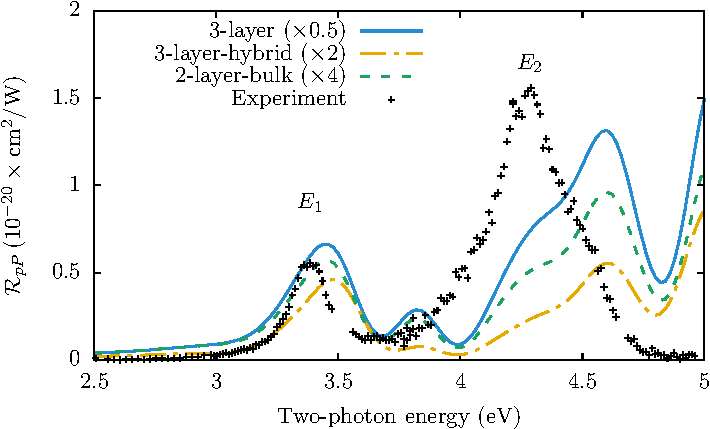
\includegraphics[width=\textwidth]{fig-Si1x1-Mejia_RpP}
\end{figure}
\column{0.5\textwidth}
\begin{figure}
\centering
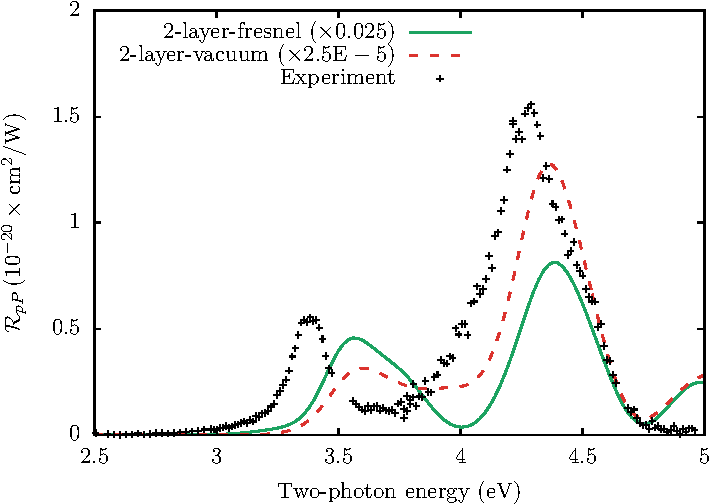
\includegraphics[width=\textwidth]{fig-Si1x1-Mejia_RpP_models}
\end{figure}
\end{columns}
\end{frame}

\end{document}
